\documentclass[10pt,a4paper]{article}
\usepackage[top=3cm,bottom=3cm,includeheadfoot]{geometry}	% Seitengeometrie festlegen
\usepackage[ngerman]{babel}
\usepackage{fancyhdr}						% das nötige Paket um Fuß- / Kopfzeilen zu verwenden			
\usepackage[utf8]{inputenc}
\usepackage{amsmath}
\usepackage{amsfonts}
\usepackage{amssymb}
\usepackage{caption}
\usepackage{listings}
\usepackage{textcomp}
\usepackage{graphicx}
\usepackage{color}
\newcommand{\hilight}[1]{\colorbox{yellow}{#1}}
\usepackage{chngcntr}
\usepackage{hyperref}
\usepackage{caption}
\usepackage{colortbl}

\counterwithin{figure}{section}

\author{Ken Hasenbank, Artur Schmidt}
\title{Praktikum 1}
\date{04.12.2017}

\makeatletter

\pagestyle{fancy}	%ermöglicht die Verwendung von eigens bearbeiteten Kopf-/ Fußzeilen
\fancyhf{}
%Bearbeiten der Kopzeile
\fancyhead[R]{\thepage}
\fancyhead[C]{Chaos \& Fraktale}
\fancyhead[L]{\@date}
\renewcommand{\headrulewidth}{0.4pt} %obere Trennlinie
%Bearbeiten der Fußzeile
\fancyfoot[C]{ \centering Ken Hasenbank,\linebreak Artur Schmidt}
\renewcommand{\footrulewidth}{0.4pt} %untere Trennlinie


\begin{document}
%\thispagestyle{empty}		% legt ein für diese Seite ein Layout fest, dass leer ist (keine Fuß-/ Kopfzeile etc) 

%%%%%%%%%%%%  DECKBLATT ANFANG   %%%%%%%%%%%%%%
\begin{titlepage}
\begin{center}
	\Large{Hochschule Darmstadt}\\
	\large{Fachbereich Informatik}
\end{center}

\vspace{1cm}
\begin{center}
	\large{Chaos und Fraktale}
\end{center}

\vspace{2,5cm}
\begin{center}
	\huge{Praktikum}\\
\end{center}

%\begin{center}
%	\Huge{\textbf{Praktikum 1}} 
%\end{center}


\vspace{6cm}
\begin{center}
{\large 
\begin{tabular}{lll}
	Semester: && SoSe 2017\\
	\vspace{1mm}\\
	Laboranten: && Ken Hasenbank\\
	&& Artur Schmidt\\
	\vspace{1 mm}\\
	Datum:	&& \@date\\
	\end{tabular} 
	}%\large beenden
\end{center}

\end{titlepage}
%%%%%%%%%%%%  DECKBLATT ENDE  %%%%%%%%%%%%%%5

\section{Punkt 1}
\begin{lstlisting}
// Sierpinski-Verwandter:  IFS-TEST.IFS
 3
 0.5  0.0   0.0  0.5  0.0  0.0
-0.5  0.0   0.0  0.5  1.0  0.0
-0.5  0.0   0.0 -0.5  0.5  1.0
-0.1  1.1  -0.1  1.1
 2    1
\end{lstlisting}

Das daraus entstehende Fraktal sieht dann wie volgt aus:

\begin{center}
	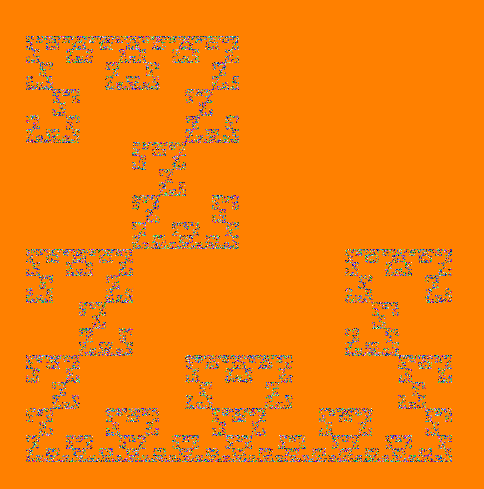
\includegraphics[scale=0.5]{images/IFS-TEST.png}
	\captionof{figure}{IFS-TEST}
	\label{fig:prim}
\end{center}

\section{Punkt 2}
Egal welchen Punkt wir als Startpunkt wählen, nach genügend Transformationen mit den in den IFS-Dateien beschriebenen Vorschriften landet er zwangsweise auf dem Attraktor. z.B. dem Sirpinski-Dreieck

\section{Punkt 3}
Da wir einen Punkt nicht mit jeder Matrix transformieren, sondern immer nur eine zufallsgesteuert Auswählen ergeben sich nicht die selben Orbist. Allerdings landen (nach einer gewissen Anzahl an Iterationen) alle generierten Punkte auf dem Attraktor.

\section{Punkt 4}
Beim Sirpinski-Dreieck ist jede Transformation dafür zuständig genau ein Drittel der Gesamtfläche zu füllen, wodurch eine faire, zufallsgesteuerte Auswahl der nächsten Transformation das richtige Ergebnis liefert. 

Beim Farn allerdings müssen die Unterschiedlichen Transformationen teils enorm unterschiedlich große Flächen zu füllen. Bei einer gleichverteilten Zufallsteuerung wird hier der stiel mit genauso vielen punkten gezeichnet wie die Blätter, wobei der Stiel nur einen Bruchteil der Fläche einnimmt.

\section{Punkt 5}

\section{Punkt 6}
\begin{lstlisting}
// Gray-Figur
 3
 0.5   0     0    0.5  0.0  0.5
 0.5   0     0   -0.5  0.0  0.5
-0.5   0     0    0.5  1.0  0.5
-0.1   1.1  -0.1  1.1
 2     1
\end{lstlisting}

Das daraus entstehende Fraktal sieht dann wie volgt aus:

\begin{center}
	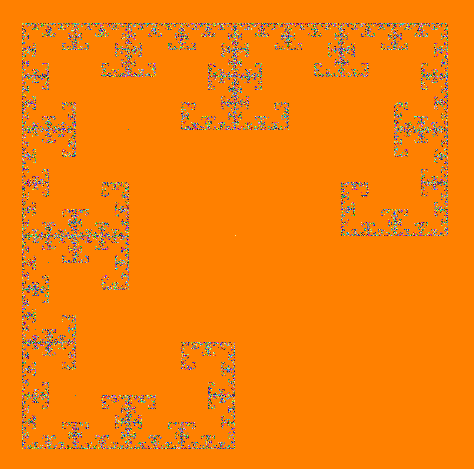
\includegraphics[scale=0.5]{images/IFS-GRAY.png}
	\captionof{figure}{IFS-TEST}
	\label{fig:prim}
\end{center}

\section{Punkt 7}


\end{document}
\makeatother